\chapter{Examinatio Sacer Basilicum (sic)}

{\itshape
Auch wenn diese Informationen natürlich nicht die Hallen der Gilden verlassen sollten, so kann ich nicht umhin, hier einen Blick hinter die Kulissen der Planung zu gewähren. Auch wenn große Teile der Gezeichneten dieses Blatt kennen, einer kennt es nicht!
}

Etwas Hintergrund (Setzungen):

Die Examinatio Sacer Basilicum findet in einer, angeblich von Basilius dem Großen selbst erschaffen (was allerdings anzuzweifeln ist) Globule statt. Dies hat den Vorteil, dass die Prüfer natürlich toll zugucken und eingreife können. Von der Beschreibung wollte ich mich an den diversen Aufnahmeprüfungen der Aes Sedai aus dem Rad der Zeit orientieren.

Accepted: 	Moralische / Seelische Prüfung\\
Aes Sedai:	Zaubern unter großen Ausnahmesituationen\\
Rhuidean:	Visionen über Zukunft und Vergangenheit

Letzteres finde ich als Prüfung weniger passend, da sie im Rad der Zeit im Kontext natürlich sehr schwierig für die Prüflinge ist, aber ich wüsste nicht, was man Temyr zeigen kann, was ihn groß schocken und in eine Sinnkrise führen würde. Außer Aria, die von Firnen vergewaltigt wird, aber ich glaube das Territorium will keiner betreten.\footnote{Uff, das habe ich geschrieben??? \~ Claas}

Eine Rätsel/Zauberprüfung gemischt mit einigen moralischen Entscheidungen gefällt mir eigentlich, genauso wie der Vorschlag, dass jeder Prüfer eine der Prüfungen (mit)gestaltet. Dann stelle ich mir so etwas wie folgendes vor:

\paragraph{Racalla von Horsen-Rabemund:} Göttertreue und Rätsel -- kein Plan
\paragraph{Prishya von Garlischgrötz:} analytisches Denken und klares Handeln -- a la Harry Potter 1: die Zaubertränke, das Hermine löst
\paragraph{Salpikon Savertin:} Handeln unter Druck und Kreativität -- schwieriges Logikrätsel um durch eine Tür zu kommen, in der Mitte hockt ein Dämon mit einem Schlüssel und der Raum füllt sich mit Wasser
\paragraph{Rohezal vom Amboss:}	Weisheit -- Salomonisches Urteil
\paragraph{Robak von Punin:} wissenschaftliches Arbeiten und analytisches Denken -- ähnlich wie Prishya (?)
\paragraph{Thomeg Atherion:} TROLOLOLOLOLOL -- Entweder viel zu einfach oder völlig unlösbar: besiege diese hundert Zants und iss diesen Apfel besonders erotisch
\paragraph{Rakorium Muntagonus:} muss auch irgendwie haarsträubend schwierig werden -- Jetzt mit tausend Echsen!!!

Das ist ein grober Entwurf. Ich beanspruche für mich auf jeden Fall die Figur des Rohezal, alle anderen können wir aufteilen. Keiner spricht spontan Firnen während der Prüfung frei!!! Die Wahl zum Erzmagier muss danach ohne Gegenstimme erfolgen. Nach der Prüfung darf jeder Prüfer, so er es will, dem Prüfling noch eine Frage stellen, nach der er entscheidet, ob der Prüfling den Rang eines Archomagus verdient hat oder nicht.

Bei der Wahl des Gremiums fällt auf, dass keine expliziten Feinde der Gezeichneten nominiert sind. Beide Schwarzmagier gehören dem Antiborbaradianischen Flügel an, die Graumagier sind, mit Ausnahme von Robak von Punins, Temyr gegenüber poitiv eingestellt, und auch letzterer ist einfach nur auf die Erhaltung des übermenschlichen Anspruchs bedacht, den die Basiliusprüfung darstellt. Die Weißmagier sind beide keine Fanatiker, Racalla von Horsen-Rabmund denkt genauso wie Robak, während Rohezal als Neorohalist natürlich streng gegen Borbarad kämpft und die Gezeichneten nach Kräften unterstützen will.

\chapter{Die Enduriumwaffen}

\section{Der Degen des Firnen Wulfgrimm: Vulnus}
\begin{figure*}[b]
    \centering
    \begin{minipage}{0.3\linewidth}
    \centering
    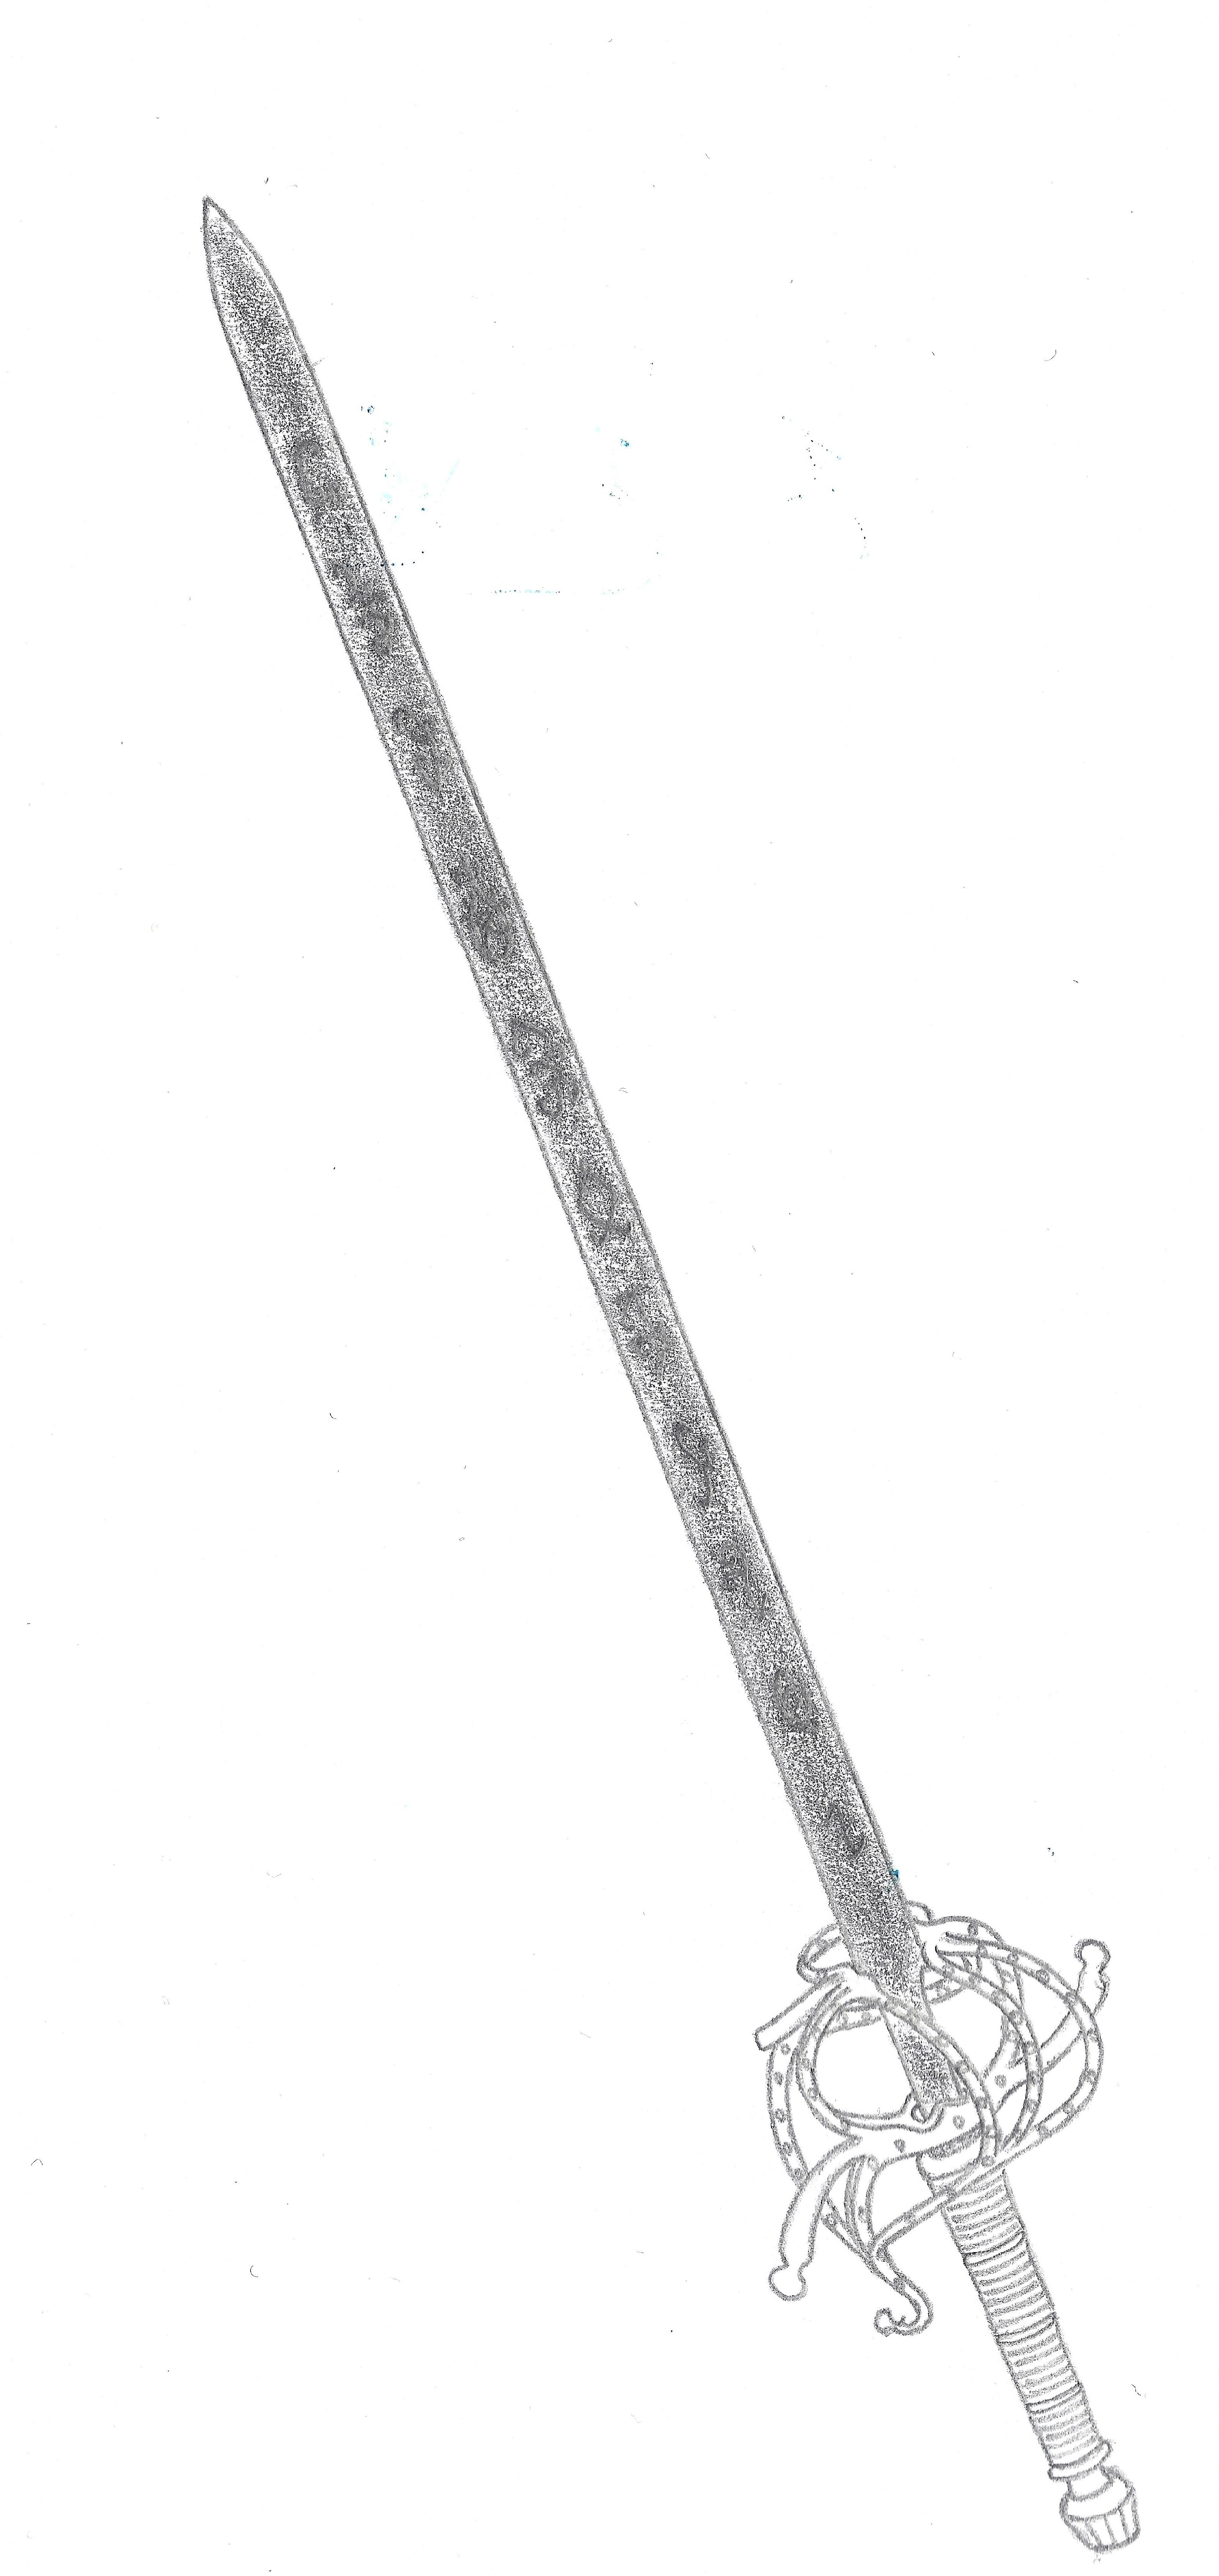
\includegraphics[width=\textwidth]{illustrations/firnen_endurium.jpg}
    \end{minipage}
    \begin{minipage}{0.3\linewidth}
    \centering
    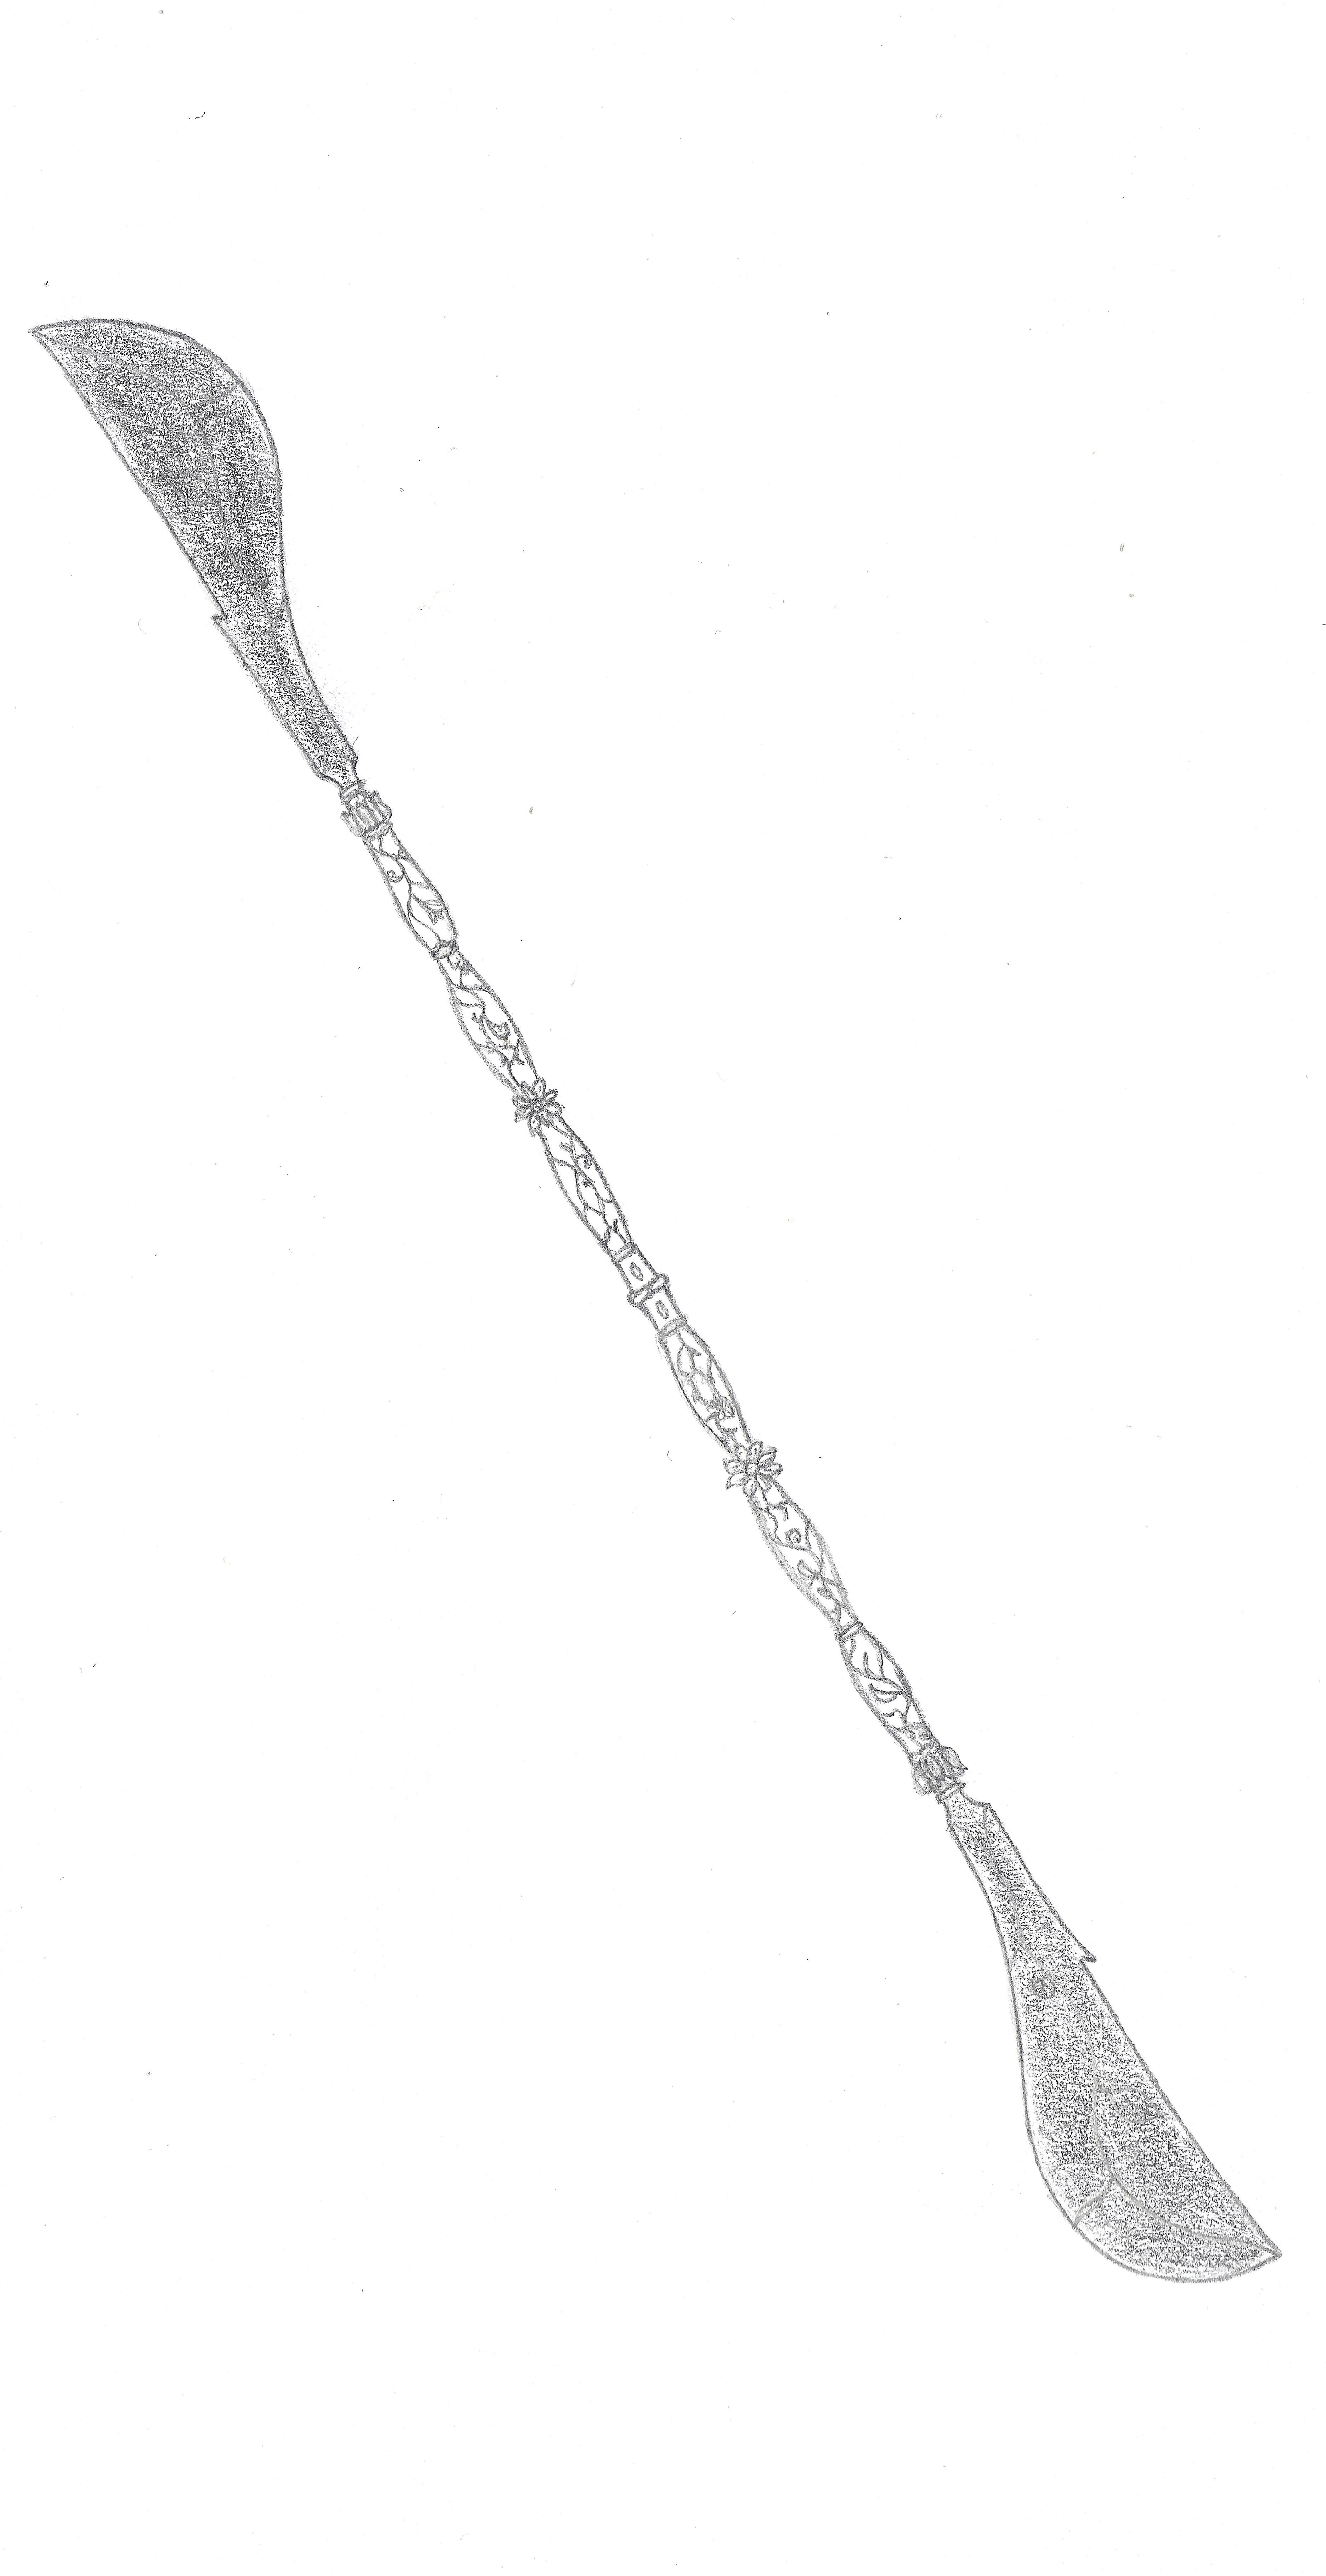
\includegraphics[width=\textwidth]{illustrations/toran_endurium.jpg}
    \end{minipage}
    \begin{minipage}{0.3\linewidth}
    \centering
    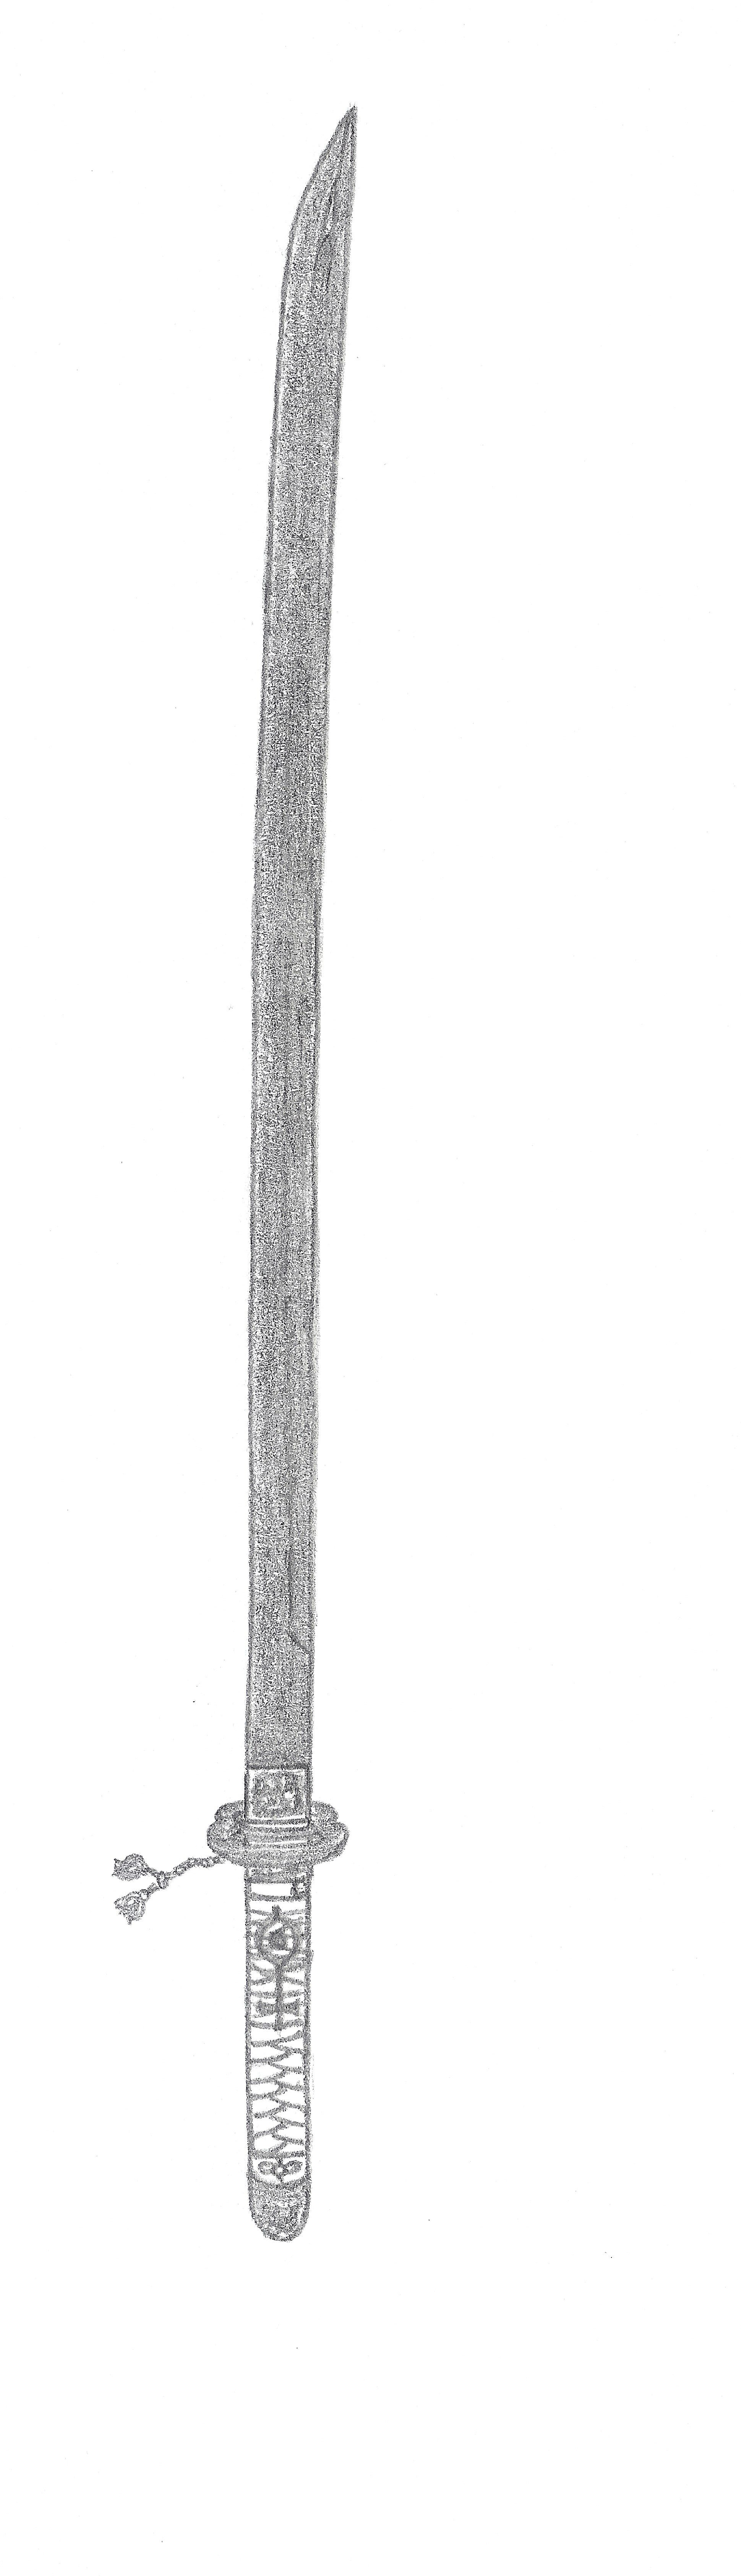
\includegraphics[width=0.6\textwidth]{illustrations/rezzanjin_endurium.jpg}
    \end{minipage}
\end{figure*}

\paragraph{Aussehen}
Der lange Magierdegen wurde aus feinstem Endurium gefertigt. Die Intarsien sind aus Mondsilber und bilden Schutz- und Bannglyphen in den magischen Runen des Arkanil. Das Heft ist von einem Kunstvollen Korb umflochten, der mit kleinen Quarzen besetzt ist.

\paragraph{Herstellung}
Das etwa ein Schritt lange Schwert ist ein Meisterwerk der Feinschmiedekunst, erschaffen von Sephira Eisenlieb, einer einfachen und doch begnadeten Geweihten des Ingerimm aus Angbar. 

\paragraph{Weihe}
Schwester Eisenlieb weihte das Werk permanent dem Ingerimm im Tempel des Ingerimm zu Angbar.


\section{Die Zweililie des Toran Ostik: Zahrabel, Blüte der Herrin}

\paragraph{Aussehen:}
Der Stab liegt schwerer in deiner Hand als dein alter, und ist aus dunklem Eichenholz gefertigt. Die Klingenblätter an beiden Enden glänzen schwarz und die Griffstange ist mit einem filigranen Geflecht aus geschnitzten Ranken und Blumen verziehrt. 

\paragraph{Herkunft:}
Der Stab der Waffe wurde dem Tsapriester Zadikar von Borbra von einem Elfen geschenkt, die Klingen wurden von einem Grangorer Meisterschmied gefertigt.

\paragraph{Weihe:}
Bruder Zadikar weihte die Zweililie permanent seiner Göttin um gegen die Pervertierung des Lebens stehen zu können.

\section{Das Schwert des Rezzanjin Al'Ahjan: Seyf, Schwert}

\paragraph{Aussehen:}
Das schwere Tuzakmesser ist etwas länger als üblich und aus tiefschwarzem Endurium gefertigt. Rote und Goldene Intarsien ziehen sich über die Klinge, wie Blut und geben der Waffe ein fließendes Aussehen. Der Griff ist mit rotem Leder umwickelt und mit goldenem Draht gesichert. Der Knauf wird von einem goldenen Löwenkopf geziert. 

\paragraph{Herkunft:}
Der Erschaffer dieses Meisterwerks ist der maraskanische Exilant Mulziber von Tuzak, der Schüler und Erbe des legendären Meisterschmiedes Grijomacon, der einst das Kaiserschwert Silpion erschuf.

\paragraph{Weihe:}
Die Erhabene Ayla von Schattengrund weihte die Waffe in einer Zeremonie feierlich permanent der leuengleichen Göttin Rondra.

\section{Der Bogen des Ragnos vom Svelltal: Cúnamorn ar Cún'anga}

\paragraph{Aussehen:}
Der mächtige Kriegsbogen ist aus Steineiche gefertigt und größer als alle Bögen, die du bisher geführt hast. Der Griff und die Spitzen sind mit schwarzem Endurium beschlagen. Beide Hörner des Bogens gleichen den Hörnern des Drachen, den du in deinem jetzt schon legendären Kampf vertrieben hast.
Köcher mit hundert enduriumbestückten Pfeilen liegen bei, sowie sieben Pfeile mit roten Federn, die in eine Rehhaut eingeschlagen sind.

\paragraph{Herkunft:}
Der Bogen wurde vom Roten Pfeil, Tenobaal Totenamsel, aus einer Steineiche gefertigt und von einem elfischen Schmied aus Donnerbach mit Endurium verziehrt.

\paragraph{Weihe:}
Der Bogen wurde durch einen unbekannten Firunpriester permanent dem Grimmigen Wintervater geweiht.

\section{Das Schwert des Arngrimm von Ehrenstein: Wolfsklaue}

\paragraph{Aussehen:}
Das lange, schlanke Bastardschwert ist wie seine Geschwisterwaffen aus tiefschwarzem Endurium gefertigt. Die Klinge ist gerade und so perfekt glatt, dass sich trotz der Schwärze des Stahl dein Gesicht darin spiegelt, als du es ziehst. 
Das Heft ist aus Ebenholz gefertigt und mit Silber und Elfenbein beschlagen. Den Knauf ziehrt ein weißer Wolfskopf, dessen gelbe Augen glatt polierte Bernsteine sind.

\paragraph{Herkunft:}
Thorn Eisinger, der bekannteste Waffenschmied Gareths schmiedete das Schwert für den heldenhaften Spross des Hauses Eherenstein aus dem in Maraskan geraubten Endurium.

\paragraph{Weihe:}
Das Schwert wurde vom Raben persönlich in einer stillen Zeremonie dem Gott Boron permanent geweiht.

\begin{figure*}[b]
    \centering
    \begin{minipage}{0.3\linewidth}
    \centering
    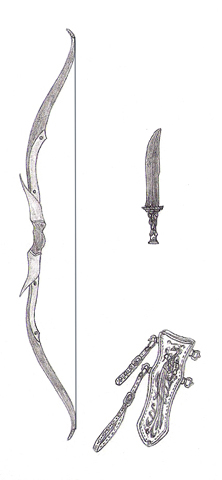
\includegraphics[width=\textwidth]{illustrations/ragnos_endurium.jpg}
    \end{minipage}
    \begin{minipage}{0.3\linewidth}
    \centering
    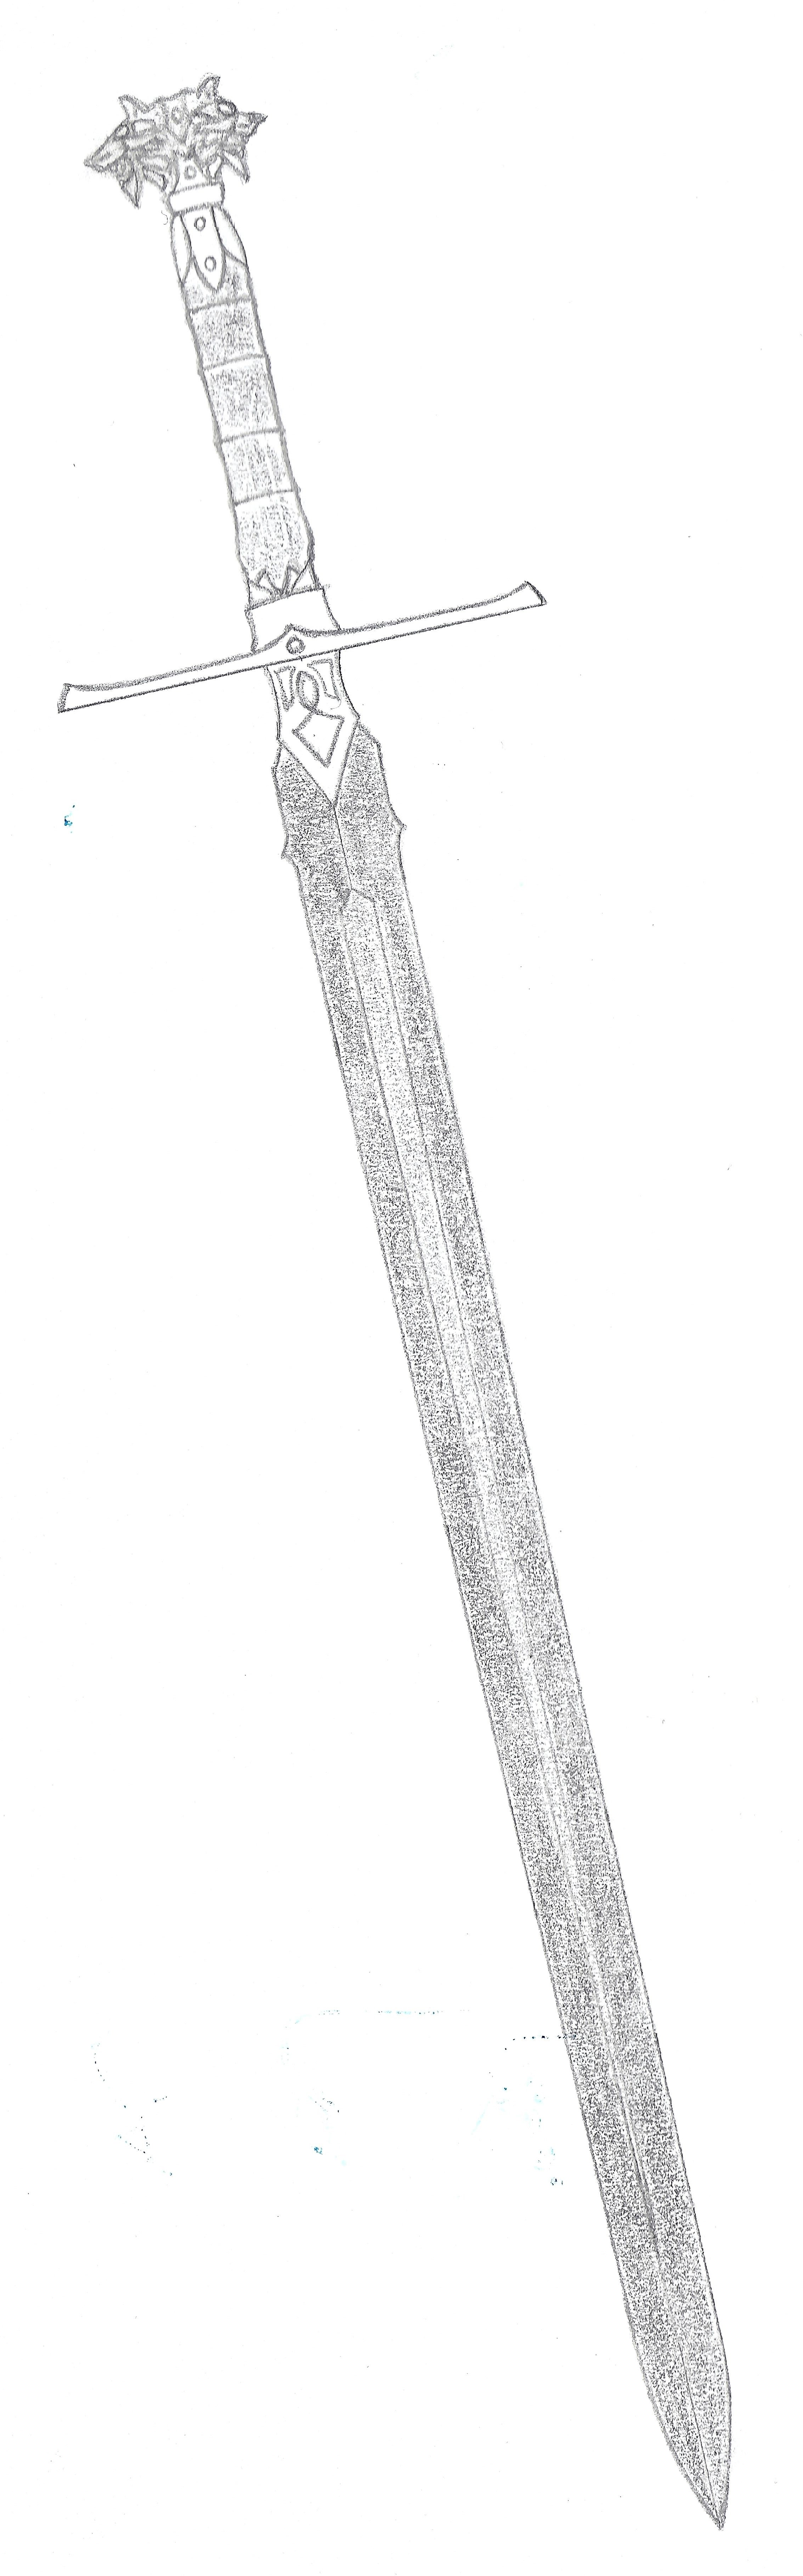
\includegraphics[width=0.6\textwidth]{illustrations/irian_endurium.jpg}
    \end{minipage}
\end{figure*}

\newpage
\FloatBarrier

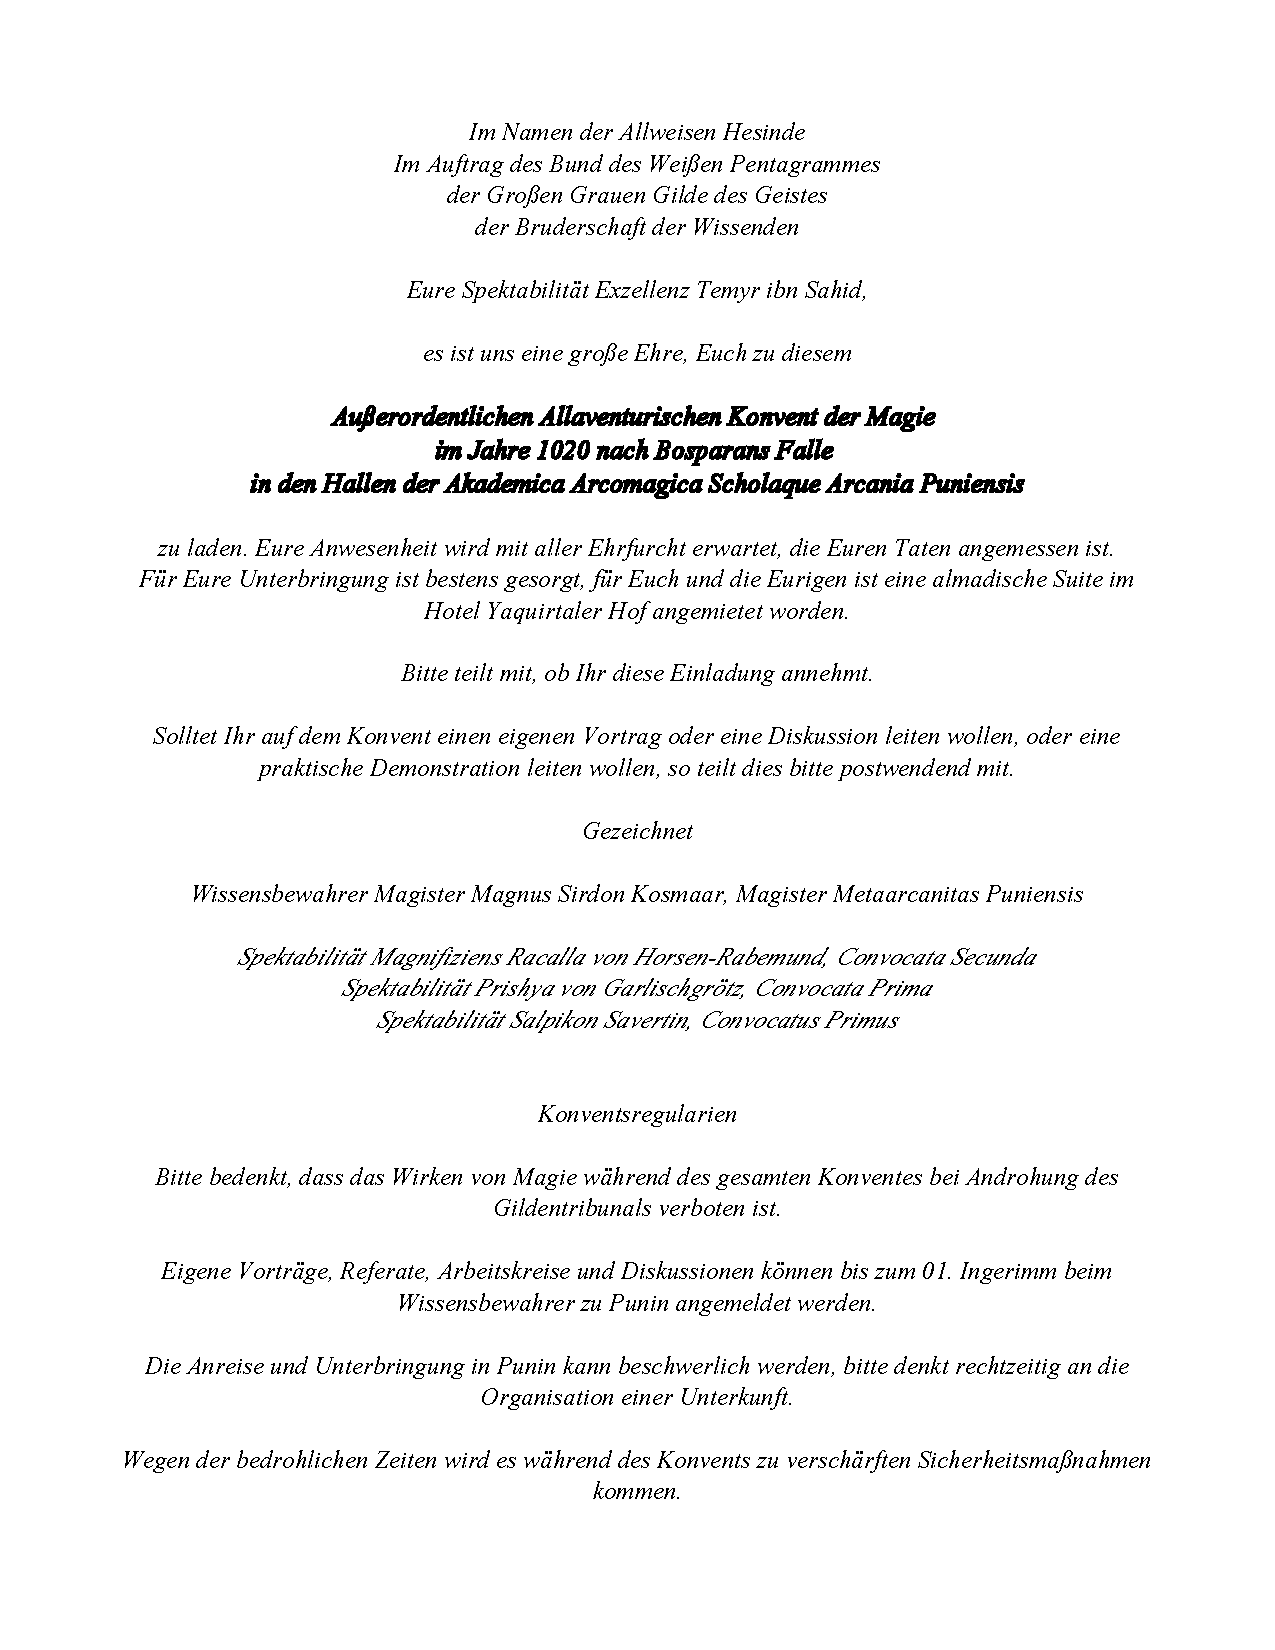
\includepdf[scale=0.9,pages=1]{handouts/part_4/rv_einladung_magierkonvent.pdf}
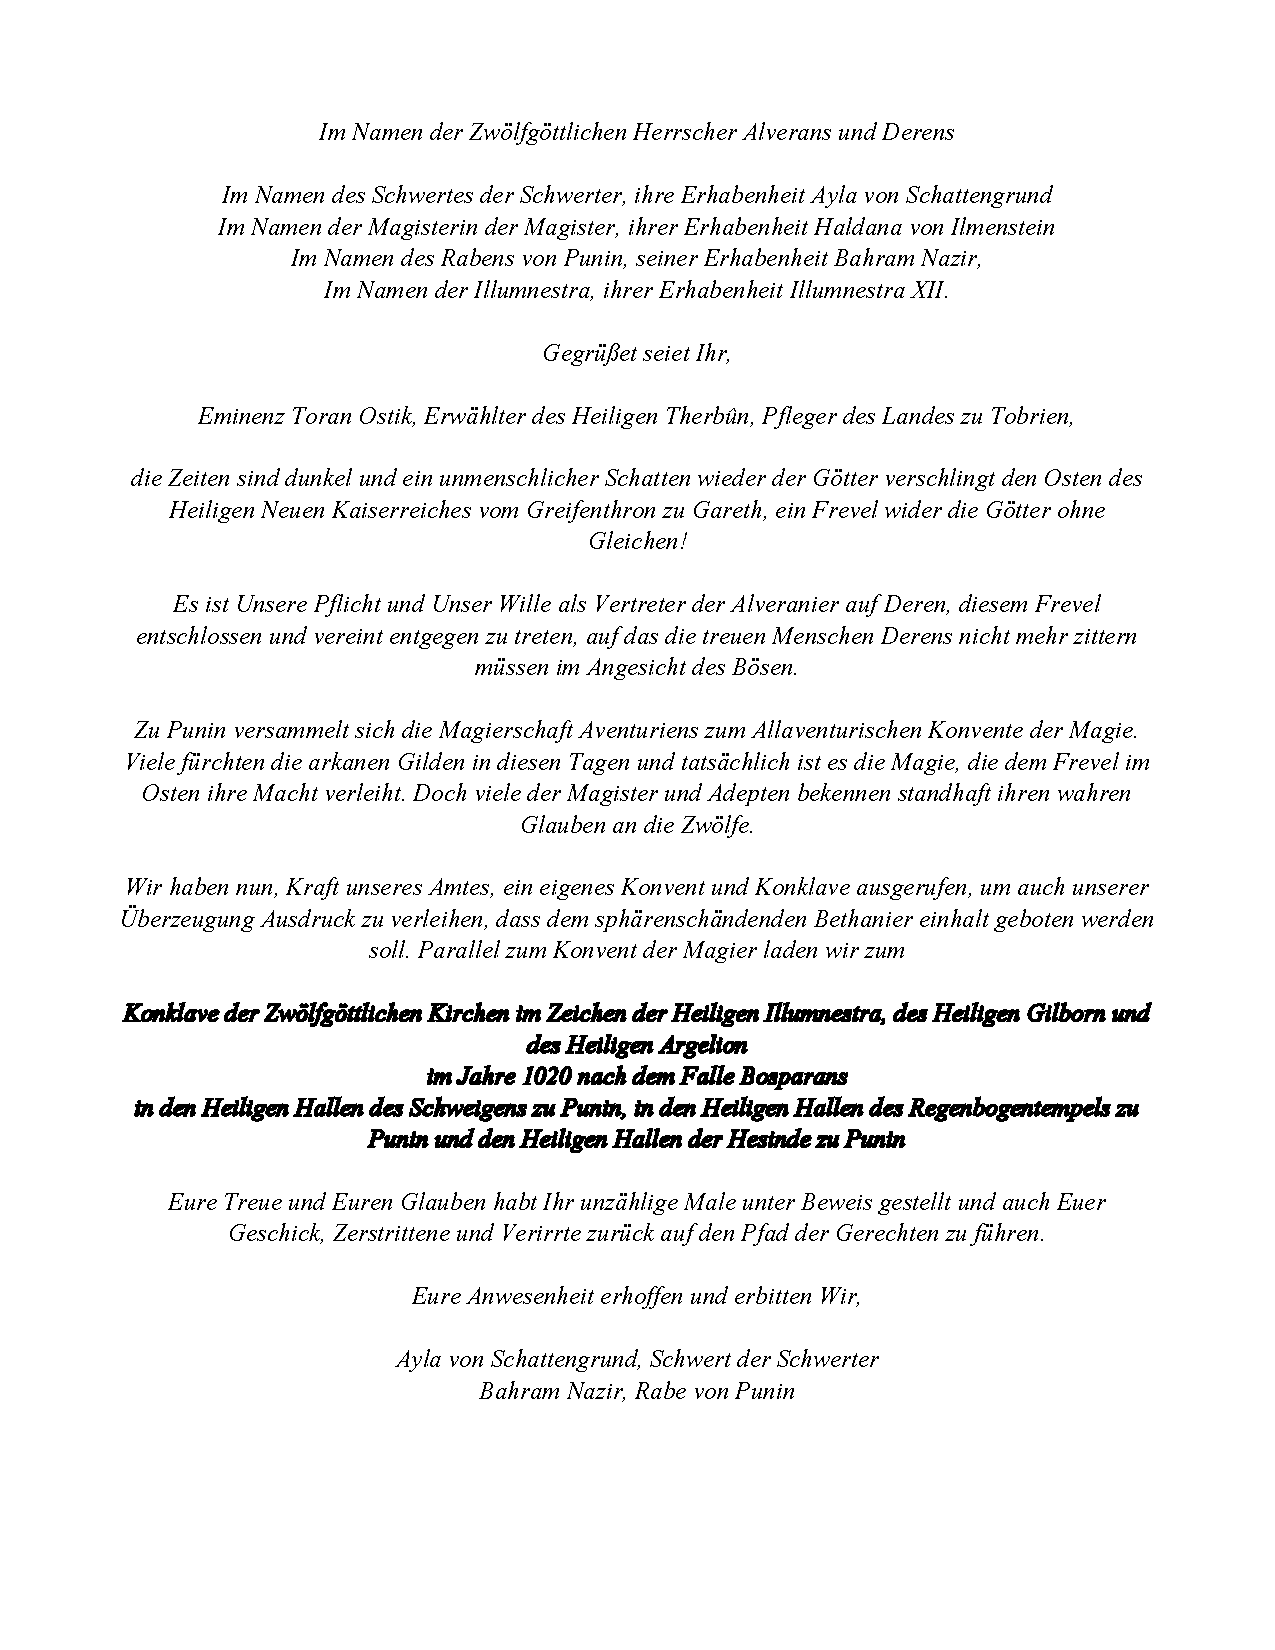
\includepdf[scale=0.9,pages=-]{handouts/part_4/rv_einladung_toran.pdf}
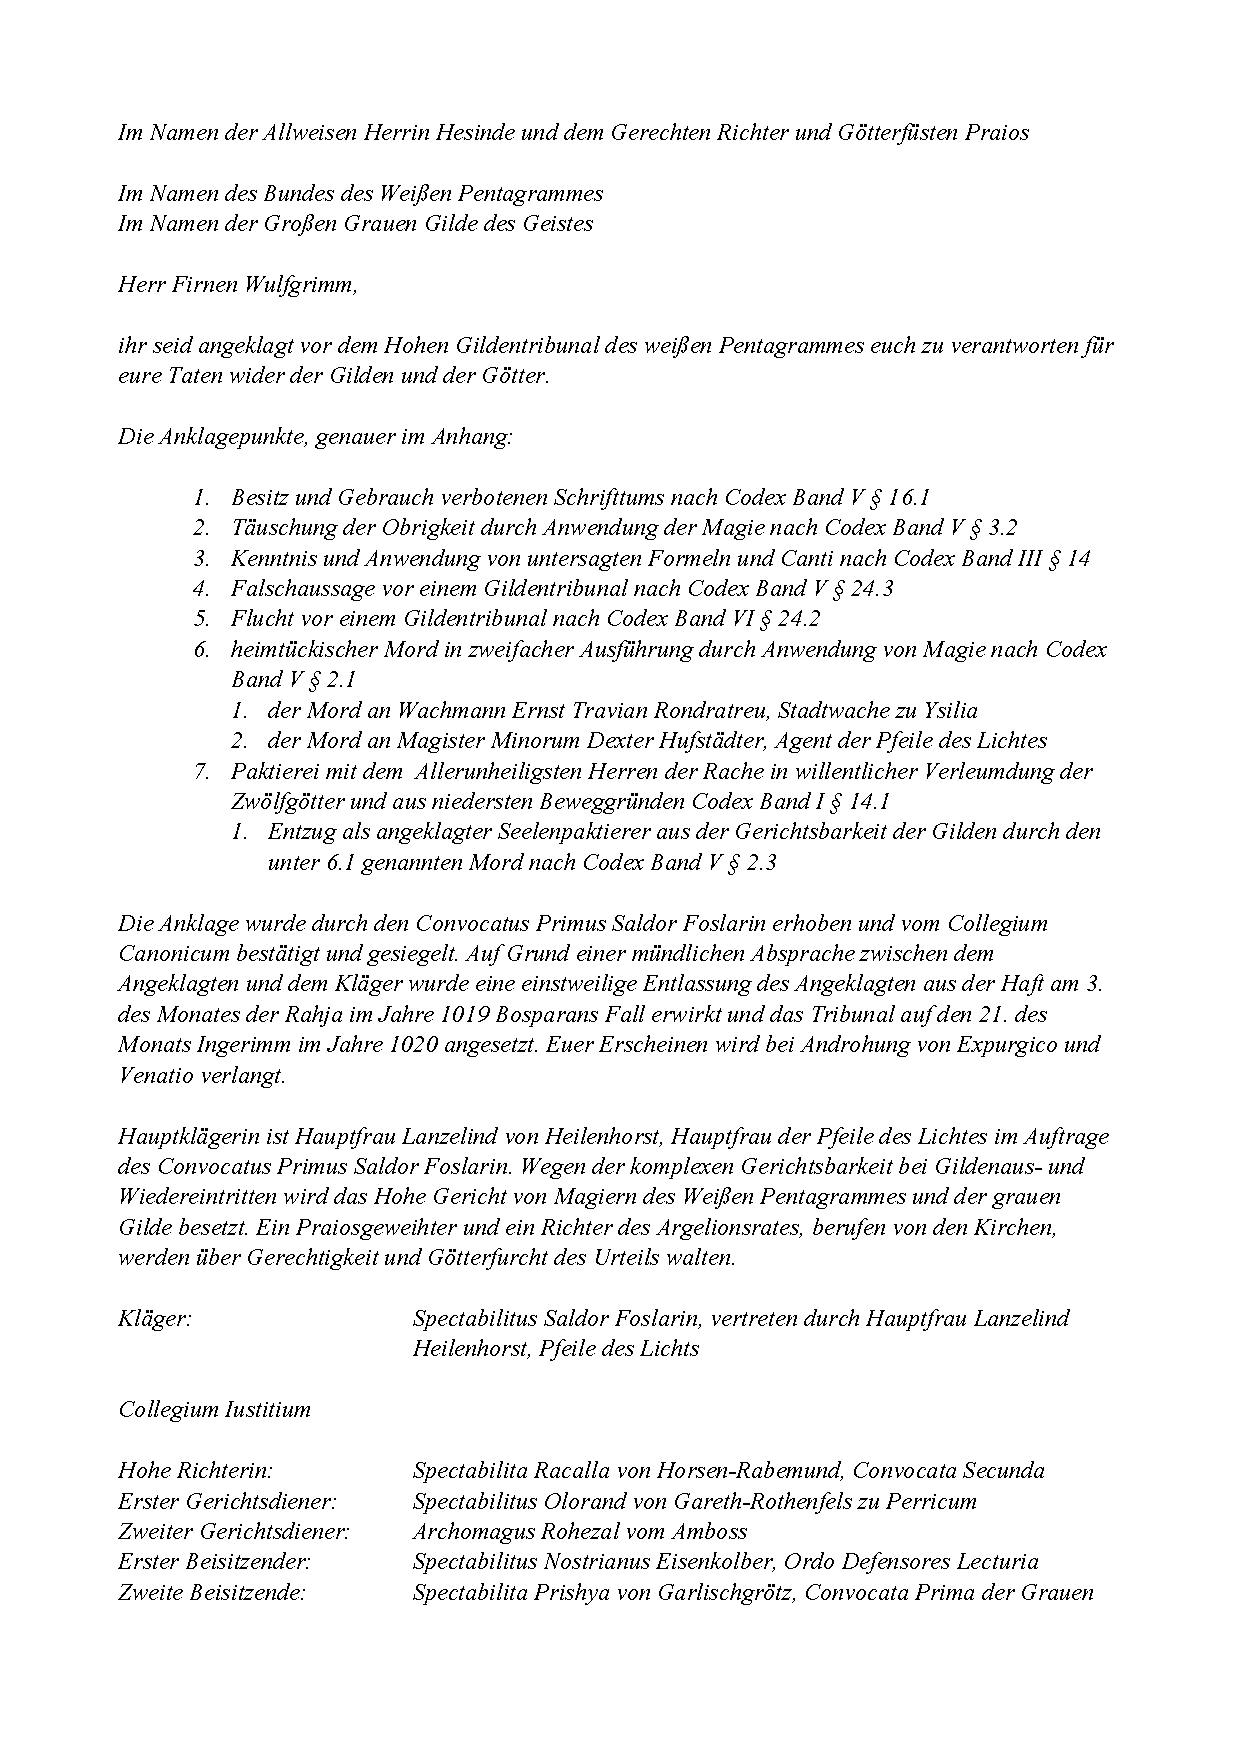
\includepdf[scale=0.9,pages=-]{handouts/part_4/rv_vorladung_firnen.pdf}
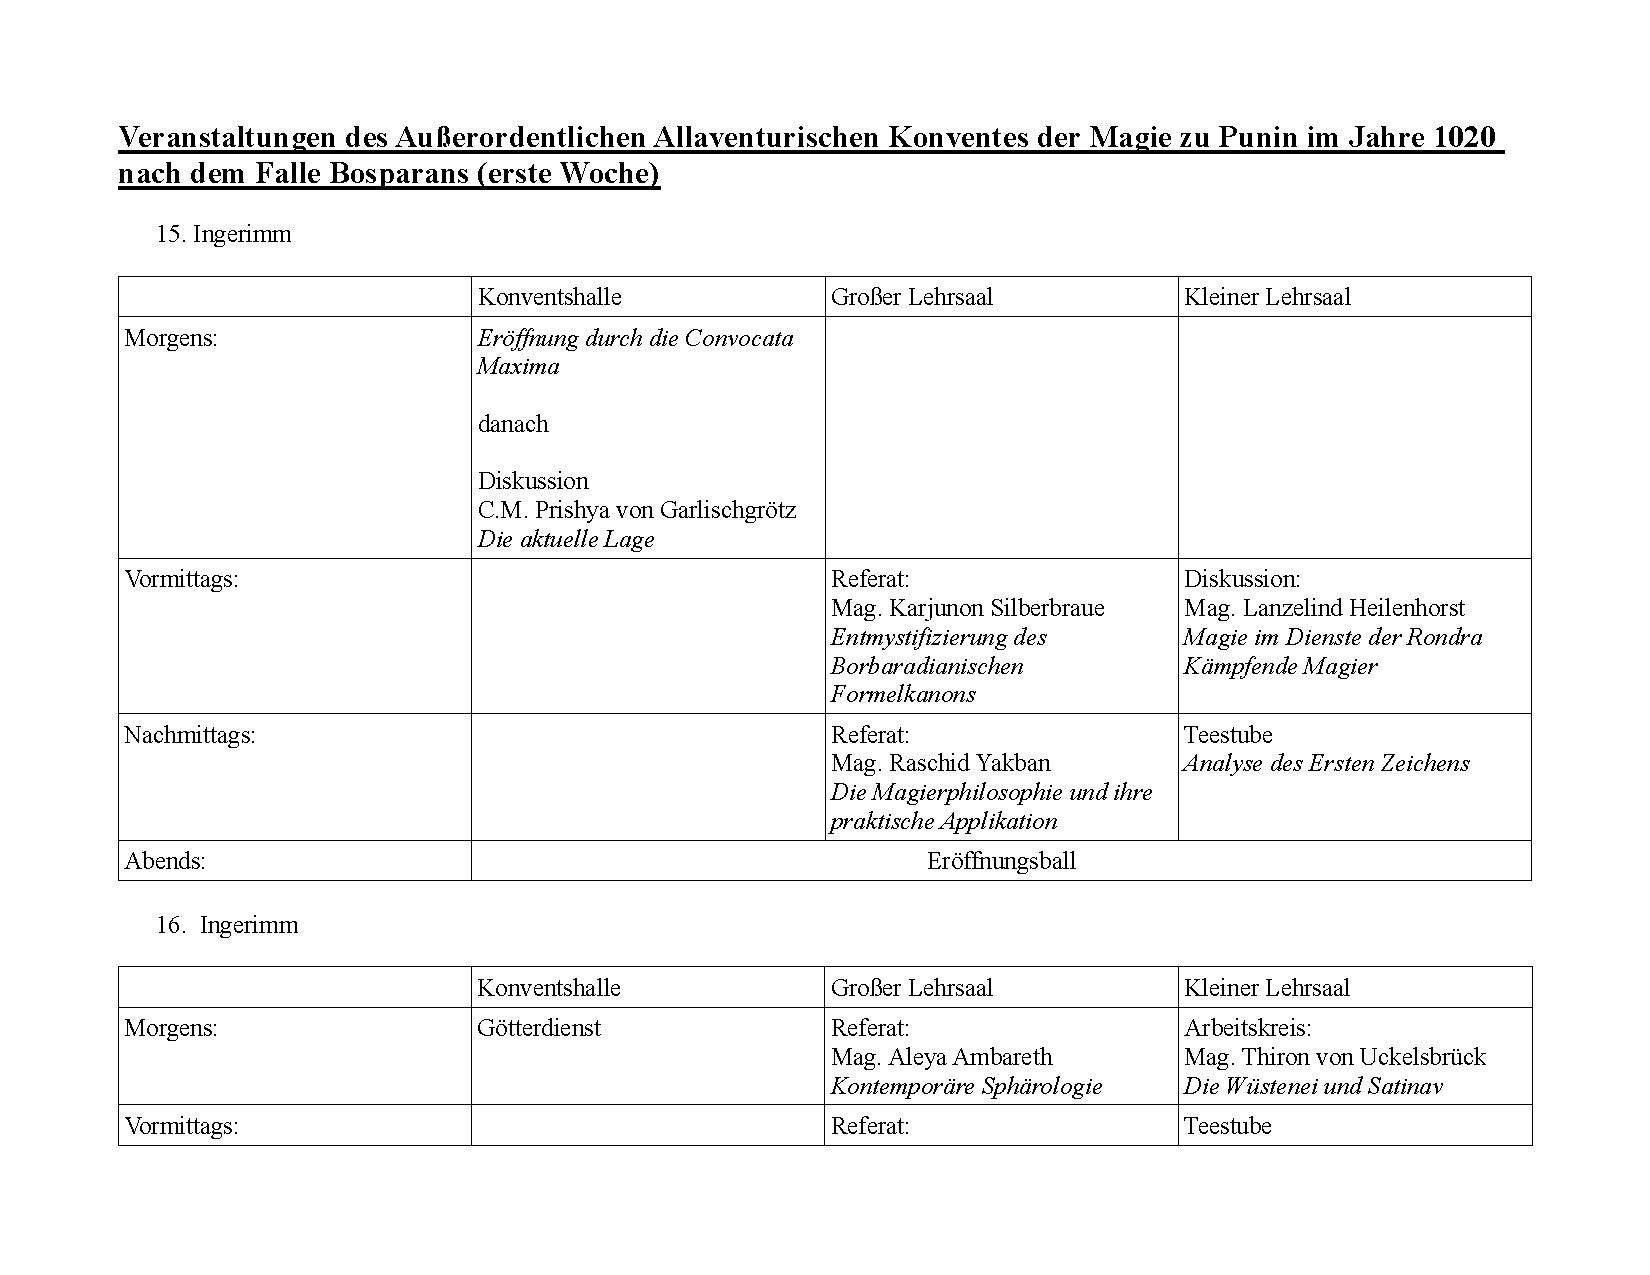
\includepdf[scale=1.0,pages=-,nup=1x2]{handouts/part_4/rv_tagesordnung.pdf}